\documentclass{article}

\usepackage{spconf,amsmath,amssymb,amsthm,graphicx,booktabs,multirow,array,hyperref}
\usepackage{algorithm,algorithmic}
\usepackage{placeins}
\usepackage{balance}
\usepackage{microtype}
\usepackage[T1]{fontenc}

\hypersetup{hidelinks,hypertexnames=false}

\newtheorem{definition}{Definition}
\newtheorem{theorem}{Theorem}
\newtheorem{lemma}{Lemma}
\newtheorem{proposition}{Proposition}
\newtheorem{corollary}{Corollary}
\newtheorem{remark}{Remark}

% Smaller hollow square as the end-of-proof marker (adjust the scale factor
% to taste; .7 keeps it clearly smaller than the default box).
\newcommand{\whitesquare}{\ensuremath{\scalebox{.7}{$\square$}}}
\renewcommand{\qedsymbol}{\whitesquare}

\newcommand{\R}{\mathbb{R}}
\newcommand{\supp}{\operatorname{supp}}
\newcommand{\dist}{\operatorname{dist}}
\newcommand{\eps}{\varepsilon}
\newcommand{\Peta}{\mathcal{P}_{\eta}}
\newcommand{\Top}{\operatorname{Top}}

% Keep the official ICASSP margins and font sizes.  Space is recovered by
% shortening exposition, merging floats, and reducing figure height rather
% than by changing the template geometry.
\setlength{\textfloatsep}{4pt plus 1pt minus 1pt}
\setlength{\floatsep}{3pt plus 1pt minus 1pt}
\setlength{\intextsep}{3pt plus 1pt minus 1pt}

% Compact author block: drop the blank row after the name row and tighten the
% title area (official fonts/margins unchanged; needed for the 4-page limit).
\makeatletter
\def\name#1{\gdef\@name{{\em #1}}}
\def\@maketitle{\newpage
 \null
 \vskip 1em \begin{center}
 {\large \bf \@title \par} \vskip .75em {\large \lineskip .5em
\begin{tabular}[t]{c}\@name \\ \@address
 \end{tabular}\par} \end{center}
 \par
 \vskip 1em}
\makeatother

\title{CERTIFIED ZEROTH-ORDER EXACT PENALIZATION FOR BLACK-BOX SPARSITY-CONSTRAINED OPTIMIZATION}

\name{Dongxu Liu$^{1,*}$\thanks{$^{*}$Corresponding author.}, Dongyang Liu$^{2}$, Wenjia Shi$^{3}$, Keming Fan$^{3}$, Linhao Wang$^{3}$}
\address{$^{1}$School of Artificial Intelligence, Jilin University, Changchun, China\\
$^{2}$Yingcai Honors College, University of Electronic Science and Technology of China, Chengdu, China\\
$^{3}$College of Computer Science and Technology, Jilin University, Changchun, China\\
{\scriptsize E-mail: liudx9924@mails.jlu.edu.cn, 2024310102018@std.uestc.edu.cn, shiwj2126@mails.jlu.edu.cn, fankm2124@mails.jlu.edu.cn, lhwang2124@mails.jlu.edu.cn}}

\begin{document}
\ninept
% \ninept switches to \small, which resets the display skips of article.cls;
% tighten them afterwards so that the enlarged Figure~1 fits the 5-page limit.
\setlength{\abovedisplayskip}{4pt plus 1pt minus 1pt}
\setlength{\belowdisplayskip}{4pt plus 1pt minus 1pt}
\setlength{\abovedisplayshortskip}{3pt plus 1pt}
\setlength{\belowdisplayshortskip}{3pt plus 1pt minus 1pt}
\maketitle
\vspace{-0.75em}

\begin{abstract}
Exact-penalty methods reformulate sparsity into continuous objectives, but existing trimmed-$\ell_1$ algorithms rely on first-order proximal updates and do not directly apply to function-value-only black-box problems. We propose ZO-IDEP, a zeroth-order realization of this exact-penalty route using coordinate finite differences and the closed-form trimmed-$\ell_1$ proximal map. To our knowledge, it is the first ZO treatment of this route that certifies when inactive coordinate queries become permanently redundant. The key analysis propagates estimator error through convergence and identification. We prove convergence to a sparse proximal fixed point, finite support identification, and, under convexity of the restricted objective plus a valid localization radius, trajectory-preserving support restriction, after which the restricted and hypothetical full-coordinate trajectories coincide, reducing per-step queries from $2d$ to $2k$. Experiments verify exact post-switch step preservation, $58.3$--$62.5\%$ finite-budget savings, and the failure of heuristic early freezing.
Code is available at \url{https://github.com/ldx825/ZO-IDEP_ICASSP-2027}.
\end{abstract}

\begin{keywords}
zeroth-order optimization, exact penalty, sparse optimization, support identification, black-box optimization
\end{keywords}

\section{Introduction}
Consider the cardinality-constrained problem
\begin{equation}
    \min_{x\in\R^d} f(x) \quad \text{s.t.}\quad \|x\|_0\le k.
    \label{eq:l0}
\end{equation}
Sparse optimization is classically approached through convex and nonconvex regularization \cite{tibshirani1996lasso,fan2001variable,zhang2010mcp} or explicit subset selection \cite{bertsimas2016bestsubset}. Zhao \emph{et al.} recently developed an exact-penalty route based on
\begin{equation}
    \Phi_\lambda(x)=f(x)+\lambda h_k(x),\qquad
    h_k(x)=\|x\|_1-\|x\|_{[k]},
    \label{eq:penalty}
\end{equation}
where $\|x\|_{[k]}$ sums the $k$ largest magnitudes \cite{zhao2026exact}. Under their error-bound premise (e.g., globally $K$-Lipschitz $f$ and $\lambda>K$), the penalized and constrained solution sets coincide; related Ky-Fan/DC exact penalties appear in \cite{gotoh2018dc,yagishita2026exact}.

The missing piece is a black-box realization. Function-value-only problems arise in score APIs, auditing, and simulation \cite{chen2017zoo,vo2024brusle}. Zeroth-order (ZO) methods replace $\nabla f$ by query-based estimators \cite{nesterov2017random,ghadimi2013stochastic,duchi2015optimal,berahas2022comparison}, but coordinate differences cost $2d$ queries per iteration. Our question is whether the sparsity structure created by the exact penalty can itself reduce this black-box cost: ZO-IDEP solves the problem with full coordinate queries first, then removes inactive queries after a verifiable support certificate.

The contribution is not a new finite-difference estimator or a new sparse projection: to our knowledge, ZO-IDEP is the first ZO treatment of the trimmed-$\ell_1$ exact-penalty dynamics that \emph{certifies when inactive coordinate queries become permanently redundant}. The proof chain is: finite-difference error $\Rightarrow$ global inexact-proximal convergence $\Rightarrow$ finite support identification $\Rightarrow$ an invariant-support certificate. After certification, the $k$-coordinate trajectory is exactly the hypothetical full-coordinate proximal trajectory, reducing each future step from $2d$ to $2k$ queries.

\section{Relation to Prior Work}
\subsection{Exact penalization and a black-box oracle}
The error-bound analysis of \cite{zhao2026exact} gives equivalence of the original and penalized minimizers when $f$ is globally $K$-Lipschitz and $\lambda>K$; this premise is separate from (A1)--(A4) and the local conditions used by our theorems. Related Ky-Fan/DC penalties were studied in \cite{gotoh2018dc}, and exactness at stronger stationarity notions in \cite{yagishita2026exact}. Derivative-free penalty methods for cardinality- and mixed-integer-constrained black-box problems follow trust-region, decomposition, or active-set routes \cite{lapucci2021convergent,giuliani2022derivativefree,giovannelli2022mixed}, without a query-redundancy certificate.

\begin{definition}[Black-box oracle]
A zeroth-order oracle returns $\mathcal O_0(x)=f(x)$ for a requested $x$ but does not expose $\nabla f(x)$ or an unbiased gradient estimator.
\end{definition}

This model includes score-only neural-network access \cite{chen2017zoo,vo2024brusle} and hidden-feature sparse learning \cite{wang2026auc}.

\subsection{What is different from sparse ZO and safe screening}
Hard-thresholding methods impose sparsity at every iteration; IHT is a classical first-order example \cite{blumensath2007iht}, while SZOHT studies its interaction with ZO gradient error and may obtain weak dimension dependence \cite{devazelhes2022zeroth}; compositional stochastic thresholding targets nonlinear sparse AUC \cite{wang2026towards}. ZORO instead exploits sparsity of the \emph{gradient} \cite{cai2022zoro}, and block-coordinate ZO reduces per-step cost by querying blocks rather than an identified support \cite{cai2021zobcd}. ZO-SCHT recently combines ZO estimation with compositional hard thresholding for black-box sparse AUC optimization \cite{wang2026auc}. Generic ZO proximal methods treat broader nonsmooth black-box composites \cite{kazemi2024efficient,kungurtsev2021zeroth}.

Gap-Safe screening rules eliminate variables using convex dual regions \cite{ndiaye2017gapsafe}, and derivative-free methods identify active constraints of explicit constrained problems \cite{lewis2009active,brilli2026complexity}. Support/activity identification is also known for forward--backward and inexact proximal-gradient methods \cite{liang2017activity,dai2022inexact}, but without the black-box oracle-restriction certificate studied here. A concurrent preprint searches directly on sparse manifolds with support stabilization \cite{kimiaei2026rzcw}. ZO-IDEP instead certifies a \emph{latent Top-$k$ support generated by a nonconvex exact penalty} and proves equality between the support-restricted and hypothetical full-coordinate proximal trajectories.

\section{ZO-IDEP from Function Values}
For $z\in\R^d$, let
\begin{equation}
\Peta(z)\in\arg\min_u\left\{\lambda h_k(u)+\frac{1}{2\eta}\|u-z\|_2^2\right\}.
\label{eq:proxmap}
\end{equation}
If $I$ indexes any $k$ largest magnitudes of $z$, every global solution has the closed form \cite{zhao2026exact}
\begin{equation}
[\Peta(z)]_i=
\begin{cases}
 z_i, & i\in I,\\
 \operatorname{sgn}(z_i)(|z_i|-\eta\lambda)_+, & i\notin I.
\end{cases}
\label{eq:proxclosed}
\end{equation}
Strict margins below remove tie ambiguity.

Given only $f(\cdot)$, ZO-IDEP uses coordinate central differences
\begin{equation}
\widehat g_{t,i}=\frac{f(x_t+\mu_t e_i)-f(x_t-\mu_t e_i)}{2\mu_t},\qquad
\xi_t:=\widehat g_t-\nabla f(x_t).
\label{eq:coordzo}
\end{equation}
This estimator-error viewpoint is standard in ZO/derivative-free analysis \cite{berahas2022comparison,ghadimi2013stochastic}.

\begin{lemma}[Coordinate finite-difference error]\label{lem:fd}
If $f$ has an $L$-Lipschitz gradient, then
\begin{equation}
 \|\xi_t\|_\infty\le \frac{L\mu_t}{2},\qquad
 \|\xi_t\|_2\le \frac{\sqrt d\,L\mu_t}{2}.
 \label{eq:zoerror}
\end{equation}
\end{lemma}
\noindent The full phase performs
\begin{equation}
 x_{t+1}\in\Peta(x_t-\eta\widehat g_t),
 \label{eq:update}
\end{equation}
using $2d$ queries. Once a support $S$ is certified, ZO-IDEP queries only $S$ and uses
\begin{equation}
 x_{t+1,S}=x_{t,S}-\eta\widehat g_{t,S},\qquad x_{t+1,S^c}=0,
 \label{eq:restrictedupdate}
\end{equation}
using $2k$ queries. The full estimator available at the switching iteration is also used to test the certificate below, so switching requires no additional oracle call; Algorithm~\ref{alg:idep} summarizes the method.

\begin{algorithm}[t]
\caption{ZO-IDEP}
\label{alg:idep}
\begin{algorithmic}[1]
\STATE \textbf{Input:} $x_0$, $k$, $\lambda$, $\eta$, $\{\mu_t\}$; valid certificate data $L$, $D_t$, $\{\eps_{t+s}\}_{s\ge0}$; $S\leftarrow\emptyset$
\FOR{$t=0,1,\ldots$}
\IF{$S=\emptyset$}
\STATE query all coordinates of $\widehat g_t$ by \eqref{eq:coordzo}
\IF{$|\supp(x_t)|=k$ and \eqref{eq:convexcert} holds at $x=x_t$}
\STATE $S\leftarrow\supp(x_t)$; $x_{t+1,S}=x_{t,S}-\eta\widehat g_{t,S}$; $x_{t+1,S^c}=0$
\ELSE
\STATE $x_{t+1}\in\Peta(x_t-\eta\widehat g_t)$
\ENDIF
\ELSE
\STATE update on $S$ as in the certified branch, querying only $\widehat g_{t,S}$
\ENDIF
\ENDFOR
\end{algorithmic}
\end{algorithm}

\section{Theory}
\subsection{Global convergence and identification}
Let a bounded level set contain the iterates. Assume (A1) $f\in C^1$ has $L$-Lipschitz gradient; (A2) $\Psi(x,r):=\Phi_\lambda(x)+r^2/2$ is lower bounded and satisfies the KL property; (A3) $0<\eta<1/L$, $\{\mu_t\}$ is nonincreasing,
$\sum_t(\sum_{j\ge t}\mu_j^2)^{1/2}<\infty$, and \eqref{eq:proxmap} is solved globally; (A4) $\sup\|\nabla f(x)\|_\infty<\lambda$ on the level set, used only to conclude $k$-sparsity. KL-based inexact descent analyses of this type are standard for forward--backward schemes \cite{attouch2013convergence,bonettini2023abstract}, while explicit gradient-error conditions in convex proximal methods appear in \cite{schmidt2011inexact}.

\begin{theorem}[Full-phase convergence]\label{thm:global}
Under (A1)--(A4), the full-coordinate sequence has finite length and converges to $x^\star$ satisfying
\begin{equation}
 x^\star\in\Peta(x^\star-\eta\nabla f(x^\star)),\qquad \|x^\star\|_0\le k.
 \label{eq:pstat}
\end{equation}
Moreover, with $a=(1-\eta L)/(2\eta)$, $c_\eta=L+\eta^{-1}$, $E_T=\sum_{t<T}\|\xi_t\|_2^2$, and $\Delta_0=\Phi_\lambda(x_0)-\inf\Phi_\lambda$,
\begin{equation}
\frac1T\sum_{t<T}\dist^2(0,\partial\Phi_\lambda(x_{t+1}))
\le \frac{4c_\eta^2\Delta_0}{aT}
+\left(2+\frac{2c_\eta^2}{a^2}\right)\frac{E_T}{T}.
\label{eq:globalrate}
\end{equation}
Hence $E_\infty<\infty$ gives an $\eps$-stationary iterate in $\mathcal O(\eps^{-2})$ iterations and $\mathcal O(d\eps^{-2})$ function evaluations.
\end{theorem}

For exact $k$-sparsity, let $S^\star=\supp(x^\star)$ and
\begin{align}
\gamma_\star&=\min_{i\in S^\star}|x_i^\star|-\eta\max_{j\notin S^\star}|\nabla_j f(x^\star)|,\nonumber\\
\tau_\star&=\eta\!\left(\lambda-\max_{j\notin S^\star}|\nabla_j f(x^\star)|\right),\quad
\delta_\star=\min\{\gamma_\star/2,\tau_\star\}.
\label{eq:margins}
\end{align}

\begin{theorem}[Finite support identification]\label{thm:id}
Under (A1)--(A4), if $|S^\star|=k$, $\gamma_\star>0$, $\tau_\star>0$, and
\begin{equation}
 (1+\eta L)\|x_t-x^\star\|_2+\frac{\eta L\mu_t}{2}<\delta_\star,
 \label{eq:idcond}
\end{equation}
then $\supp(x_{t+1})=S^\star$. Consequently, a finite $T_{\rm id}$ exists after which the full method keeps $S^\star$. If, for some $q_x,q_\mu\in(0,1)$ and every $t\ge t_0$,
$\|x_t-x^\star\|_2\le C_xq_x^{t-t_0}$ and
$\mu_t\le C_\mu q_\mu^{t-t_0}$, then
\begin{equation}
T_{\rm id}
\le
t_0+2+\left\lceil\max\left\{0,
\max\left\{
\frac{\log\!\frac{2(1+\eta L)C_x}{\delta_\star}}{\log(1/q_x)},
\frac{\log\!\frac{\eta LC_\mu}{\delta_\star}}{\log(1/q_\mu)}
\right\}
\right\}\right\rceil .
\label{eq:tid}
\end{equation}
\end{theorem}
Unlike forward--backward activity identification \cite{liang2017activity,dai2022inexact}, safe screening \cite{ndiaye2017gapsafe}, and derivative-free active-set rules \cite{lewis2009active,brilli2026complexity}, the identified set here is the latent Top-$k$ support of the exact-penalty prox, with the ZO perturbation shown explicitly.

\subsection{Certified support restriction}
At a candidate switching iteration $t$, let $x=x_t$, $S=\supp(x)$, and $|S|=k$. Define $f_S(u_S)=f(u_S,0_{S^c})$ and let $X_S^\star=\arg\min f_S$.

\begin{theorem}[Invariant-support certificate]\label{thm:safe}
Assume $f_S$ is convex and $L$-smooth, $X_S^\star\neq\emptyset$, and $0<\eta\le 1/L$. Suppose valid numbers $D_t$ and $\{\eps_{t+s}\}_{s\ge0}$ satisfy
\begin{equation}
 \dist(x,X_S^\star)\le D_t,\qquad
 \|\widehat g_{t+s}-\nabla f(x_{t+s})\|_\infty\le\eps_{t+s},
 \label{eq:convexbounds}
\end{equation}
with $B_t:=\sum_{s\ge0}\eps_{t+s}<\infty$ and $\bar\eps_t:=\sup_{s\ge0}\eps_{t+s}$. Set
\begin{align}
R_t&=D_t+\eta\sqrt{k}\,B_t,\nonumber\\
H_t&=\|\widehat g_{S^c}(x)\|_\infty+\eps_t+2LR_t,\nonumber\\
A_t&=\min_{i\in S}|x_i|-2R_t-\eta(LR_t+\bar\eps_t).
\label{eq:convexcertdef}
\end{align}
If
\begin{equation}
 H_t+\bar\eps_t<\lambda,\qquad
 A_t>\eta(H_t+\bar\eps_t),
 \label{eq:convexcert}
\end{equation}
then every subsequent support-restricted iterate remains on $S$, and at each such iterate the hypothetical full-coordinate ZO proximal step \eqref{eq:update} selects the same $S$ and returns exactly the same next point as \eqref{eq:restrictedupdate}. Thus inactive coordinate queries are redundant.
\end{theorem}

\begin{remark}[Localization radius]\label{rem:radius}
The certificate takes a valid radius $D_t$ as data. It can come from a compact level set, a problem-specific bound, or, when curvature information is available, the estimate $D_t\le(\|\widehat g_S(x)\|_2+\sqrt{k}\eps_t)/m$.
\end{remark}

\begin{corollary}[Post-switch rate and query ratio]\label{cor:query}
Under Theorem~\ref{thm:safe}, let $x_S^\star\in X_S^\star$ attain the bound $\|x-x_S^\star\|\le D_t$ and define $\bar x_N=N^{-1}\sum_{s=1}^{N}x_{t+s}$. Then
\begin{equation}
 f_S(\bar x_N)-f_S^\star
 \le \frac{D_t^2}{2\eta N}+\frac{R_t\sqrt{k}}{N}\sum_{s=0}^{N-1}\eps_{t+s}
 \le \frac{D_t^2/(2\eta)+R_t\sqrt{k}B_t}{N}.
 \label{eq:convexrate}
\end{equation}
Thus the post-switch function-value complexity is $\mathcal O(k/\eps)$; when the restricted objective is strongly convex, Proposition~\ref{prop:rsc} gives the geometric rate $\mathcal O(k\log(1/\eps))$. More generally, the restricted and hypothetical full trajectories are identical, so for a common post-switch hitting time $N_{\rm tar}$,
\begin{equation}
\frac{Q_{\rm IDEP}}{Q_{\rm full}}
=\frac{dT_{\rm sw}+kN_{\rm tar}}{d(T_{\rm sw}+N_{\rm tar})}
\longrightarrow \frac{k}{d}
\quad\text{as }N_{\rm tar}\to\infty.
\label{eq:ratio}
\end{equation}
\end{corollary}

\begin{proposition}[Strong-convexity specialization]\label{prop:rsc}
Under Theorem~\ref{thm:safe}, suppose $f_S$ is $m$-strongly convex with $m>0$ and $\mu_{t+s}\le\mu_t$, so Lemma~\ref{lem:fd} gives $\eps_{t+s}\le\eps_t=L\mu_t/2$ uniformly. Take the gradient-generated radius $D_t=(\|\widehat g_S(x)\|_2+\sqrt{k}\eps_t)/m$ and set
\begin{align}
q=\sqrt{1-\tfrac{2\eta mL}{m+L}},\qquad
H_t&=\|\widehat g_{S^c}(x)\|_\infty+\eps_t+2LR,\nonumber\\
R=D_t,\qquad
A_t&=\min_{i\in S}|x_i|-2R-\eta(LR+\eps_t).
\label{eq:rscdef}
\end{align}
If $qR+\eta\sqrt{k}\eps_t\le R$, $H_t+\eps_t<\lambda$, and $A_t>\eta(H_t+\eps_t)$, then the conclusions of Theorem~\ref{thm:safe} hold and the restricted trajectory contracts: with $r_s=\|x_{t+s}-x_S^\star\|_2$,
$r_s\le q^sR+\eta\sqrt{k}\sum_{j=0}^{s-1}q^{s-1-j}\eps_{t+j}$,
so if $\eps_{t+j}\le c\beta^j$, then $r_s=\mathcal O(\rho^s)$ with $\rho=\max\{q,\beta\}<1$, and for fixed $\mu_t=\mu$, $\limsup_{s\to\infty}r_s\le\eta\sqrt{k}L\mu/(2(1-q))$.
\end{proposition}

\section{Numerical Results}
We follow the sparse-regression protocol of \cite{zhao2026exact} with $30$ fixed seeds and $300$ steps. PG-EP is the first-order reference; Full-ZO-EP uses the same exact-penalty objective/prox without restriction; Coord-ZO-IHT and SZOHT-RD are hard-thresholding baselines \cite{blumensath2007iht,devazelhes2022zeroth}. All penalties use $\lambda_t=(\lambda/40)40^{\min\{1,(t+1)/C\}}$ and certification is tested only at terminal $\lambda$. Regression/scaling use $(\lambda,C,\eta,\mu_t)=(.025,100,.9/L,10^{-3})$; ridge logistic uses $\lambda=.02$, $\eta=.1/L$, and a swept fixed or geometric $\mu_t$ (stress: $C=200$); phase retrieval uses $\lambda=.10$ with $\eta=.8/L$. Least-squares central differences are exact ($\eps_t=0$); the logistic runs exercise $\eps_t=L\mu_t/2$ in \eqref{eq:convexcertdef}. The radius $D_t$ of Theorem~\ref{thm:safe} uses restricted curvature, $D_t=(\|\widehat g_S(x)\|_2+\sqrt{k}\eps_t)/m$ with $m=\lambda_{\min}(A_S^\top A_S/n)$ for the $n$-sample least-squares model and $m=.02$, the ridge coefficient, for ridge logistic.

\begin{table}[t]
\centering
\caption{$n=128,d=256,k=16$; means over 30 trials. Error: $\ell_2$ recovery error; Ov.: planted-support overlap; Qry.: function evaluations.}
\label{tab:main}
\setlength{\tabcolsep}{2pt}%
\begin{tabular}{@{}lrrrr@{}}
\toprule
Method & Obj.$\downarrow$ & Error$\downarrow$ & Ov.$\uparrow$ & Qry.$\downarrow$\\
\midrule
PG-EP \cite{zhao2026exact} & .0053 & .255 & .971 & FO\\
SZOHT-RD \cite{devazelhes2022zeroth} & .0451 & 1.526 & .573 & 30,300\\
Coord-ZO-IHT & .0182 & .857 & .783 & 153,600\\
Full-ZO-EP & .0053 & .255 & .971 & 153,600\\
ZO-IDEP & \textbf{.0053} & \textbf{.255} & \textbf{.971} & \textbf{59,568}\\
\bottomrule
\end{tabular}
\end{table}

For valid-bound regression and geometrically smoothed logistic runs, the maximum endpoint gap and post-switch shadow-step mismatch (restricted versus hypothetical full-coordinate step) are zero, and at fixed $k/d=1/16$ savings remain $58.3$--$62.5\%$ as $d$ grows (Table~\ref{tab:scale}), covering pre-switch cost and the switching iteration's full-coordinate estimate. The scaling sweep uses different seeds, explaining the small $(256,16)$ discrepancy with Table~\ref{tab:main}. In a harder regression sweep, $31/150$ runs do not certify within $300$ steps; the certificate is sufficient, not guaranteed.

\begin{table*}[t]
\small
\centering
\begin{minipage}[t]{.49\textwidth}
\centering
\caption{Fixed-ratio scaling; every row certifies in 30/30 runs.}
\label{tab:scale}
\setlength{\tabcolsep}{2pt}%
\begin{tabular}{@{}rrrr@{}}
\toprule
$(d,k)$ & Mean $T_{\rm sw}$ & ZO-IDEP / Full & Saving\\
\midrule
$(128,8)$ & 99.0 & 28,800 / 76,800 & 62.5\%\\
$(256,16)$ & 103.2 & 59,616 / 153,600 & 61.2\%\\
$(512,32)$ & 104.2 & 120,192 / 307,200 & 60.9\%\\
$(1024,64)$ & 112.5 & 256,320 / 614,400 & 58.3\%\\
\bottomrule
\end{tabular}
\end{minipage}\hfill
\begin{minipage}[t]{.49\textwidth}
\centering
\caption{Low-margin logistic stress test, $(n,d,k)=(512,128,8)$, 800 iterations; Wrong freeze: endpoint differs from Full-ZO-EP.}
\label{tab:freeze}
\setlength{\tabcolsep}{2pt}%
\begin{tabular}{@{}lrrr@{}}
\toprule
Rule & Mean switch & Wrong & Saving\\
\midrule
Stable-3 & 3.0 & 14/30 & 93.3\%\\
Stable-5 & 5.0 & 14/30 & 93.0\%\\
Stable-10 & 10.4 & 12/30 & 92.4\%\\
Certified ZO-IDEP & no switch & 0/30 & 0\%\\
Oracle-EndSupport & 119.3 & 0/30 & 79.6\%\\
\bottomrule
\end{tabular}
\end{minipage}
\end{table*}

\begin{figure*}[t]
\centering
\begin{minipage}{.32\linewidth}
\centering
\IfFileExists{figures/mu_certification.pdf}{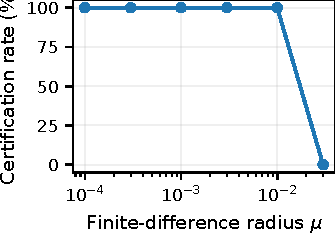
\includegraphics[width=\linewidth,height=1.45in,keepaspectratio]{figures/mu_certification.pdf}}{\fbox{\rule{0pt}{.4in}\rule{.92\linewidth}{0pt}}}\par
{(a)}
\end{minipage}\hfill
\begin{minipage}{.32\linewidth}
\centering
\IfFileExists{figures/margin_switch.pdf}{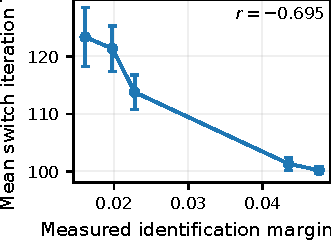
\includegraphics[width=\linewidth,height=1.45in,keepaspectratio]{figures/margin_switch.pdf}}{\fbox{\rule{0pt}{.4in}\rule{.92\linewidth}{0pt}}}\par
{(b)}
\end{minipage}\hfill
\begin{minipage}{.32\linewidth}
\centering
\IfFileExists{figures/accuracy_query_ratio.pdf}{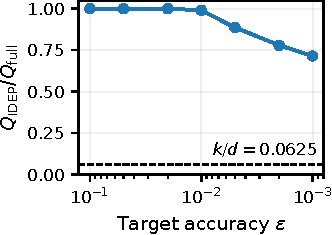
\includegraphics[width=\linewidth,height=1.45in,keepaspectratio]{figures/accuracy_query_ratio.pdf}}{\fbox{\rule{0pt}{.4in}\rule{.92\linewidth}{0pt}}}\par
{(c)}
\end{minipage}
\caption{Theory-aligned diagnostics: (a) ZO error can delay/prevent certification; (b) a larger identification margin switches earlier; (c) the query ratio decreases as the target accuracy tightens.}
\label{fig:diag}
\end{figure*}

The diagnostics (Figure~\ref{fig:diag}) agree with the theory. For $\mu\le10^{-2}$, all $30$ logistic runs certify, while at $3\times10^{-2}$ none switches; the measured identification margin correlates negatively with switch time ($r=-0.695$). Fixed-$\mu$ runs track the Proposition~\ref{prop:rsc} neighborhood; the restricted-optimum distance rises from $1.9\times10^{-10}$ to $2.3\times10^{-5}$ over the sweep. Under geometric smoothing, the empirical restricted contraction is $0.9820\pm0.0001$ for $\beta=.99$ versus the conservative $\rho=.99$ of Proposition~\ref{prop:rsc}, and $Q_{\rm IDEP}/Q_{\rm full}$ decreases from $.990$ at target $10^{-2}$ to $.715$ at $10^{-3}$. Heuristic stability rules freeze a wrong local support in $40$--$46.7\%$ of stress-test runs (Table~\ref{tab:freeze}). Phase-retrieval local-basin runs ($120/120$) satisfy the implemented certificate-form inequalities and save $48.5\%$ on average, as an empirical diagnostic with pointwise curvature surrogates.

\section{Conclusion}
ZO-IDEP makes the trimmed-$\ell_1$ exact-penalty route function-value only and propagates the ZO estimation error through convergence, identification, and certified query restriction. Once certified, inactive coordinate evaluations are provably redundant and the restricted trajectory exactly matches Full-ZO-EP. The certificate relies on a valid localization radius (Remark~\ref{rem:radius}); when the restricted objective is strongly convex, the geometric rates of Proposition~\ref{prop:rsc} apply.

\section{Appendix: Proofs}
The main proofs are collected here.
\setlength{\abovedisplayskip}{6pt plus 1pt minus 1pt}
\setlength{\belowdisplayskip}{6pt plus 1pt minus 1pt}

\medskip
\begin{proof}[Proof of Lemma~\ref{lem:fd}]
For each coordinate $i$, the fundamental theorem of calculus gives
\begin{align}
\widehat g_{t,i}-\nabla_i f(x_t)
&=\frac{1}{2\mu_t}\int_{-\mu_t}^{\mu_t}
\big(\nabla_i f(x_t+s e_i)-\nabla_i f(x_t)\big)\,ds .
\end{align}
By $L$-smoothness, the integrand is bounded in magnitude by $L|s|$, hence
$|\widehat g_{t,i}-\nabla_i f(x_t)|\le L\mu_t/2$. Taking the maximum and Euclidean norms yields \eqref{eq:zoerror}.
\end{proof}

\medskip
\begin{proof}[Proof of Theorem~\ref{thm:global}]
Let $s_t=x_{t+1}-x_t$ and $a=(1-\eta L)/(2\eta)>0$. Global optimality of the proximal subproblem, using $x_t$ as a competitor, yields
\begin{equation}
\lambda h_k(x_{t+1})+\langle \widehat g_t,s_t\rangle+\frac{\|s_t\|^2}{2\eta}
\le \lambda h_k(x_t).
\label{eq:app_prox}
\end{equation}
Combining \eqref{eq:app_prox} with $L$-smoothness of $f$, writing $\widehat g_t=\nabla f(x_t)+\xi_t$, and applying Young's inequality gives
\begin{equation}
\Phi_\lambda(x_{t+1})\le \Phi_\lambda(x_t)-\frac a2\|s_t\|^2+\frac{\|\xi_t\|^2}{2a}.
\label{eq:app_descent}
\end{equation}
Fermat's rule for the globally solved proximal subproblem provides $v_{t+1}\in\lambda\partial h_k(x_{t+1})$ such that
$\widehat g_t+s_t/\eta+v_{t+1}=0$. Therefore
\begin{align}
w_{t+1}&:=\nabla f(x_{t+1})+v_{t+1}\in\partial\Phi_\lambda(x_{t+1}),\nonumber\\
\|w_{t+1}\|&\le c_\eta\|s_t\|+\|\xi_t\|.
\label{eq:app_relerr}
\end{align}
With $\delta_t=\|\xi_t\|^2/(2a)$ and $r_t=\sum_{j\ge t}\delta_j$, set $\rho_t=\sqrt{2r_t}$ and lift to $\Psi(x,r)=\Phi_\lambda(x)+r^2/2$. Then \eqref{eq:app_descent} gives $\Psi(x_{t+1},\rho_{t+1})+(a/2)\|s_t\|^2\le\Psi(x_t,\rho_t)$. Lemma~\ref{lem:fd} and (A3) imply $\sum_t(\|\xi_t\|+\rho_t)<\infty$, while \eqref{eq:app_relerr} bounds $\dist(0,\partial\Psi(x_{t+1},\rho_{t+1}))$ by $c_\eta\|s_t\|+\|\xi_t\|+\rho_{t+1}$. These verify hypotheses H1--H4 of the abstract inexact forward--backward framework \cite{bonettini2023abstract} with $F_{\rm abs}=\Psi$, descent constant $a/2$, $b=c_\eta$, and $\zeta_{t+1}=\|\xi_t\|+\rho_{t+1}$; the KL property of $\Psi$ from (A2) supplies H5--H6 \cite{attouch2013convergence}, hence $\sum_t\|s_t\|<\infty$ and $x_t\to x^\star$. Setting $z_t=x_t-\eta\widehat g_t$ and $z^\star=x^\star-\eta\nabla f(x^\star)$, global optimality of \eqref{eq:proxmap} with arbitrary competitor $u$ gives $\lambda h_k(x_{t+1})+\frac{\|x_{t+1}-z_t\|^2}{2\eta}\le\lambda h_k(u)+\frac{\|u-z_t\|^2}{2\eta}$; passing to the limit proves \eqref{eq:pstat}. A nonzero soft-thresholded tail coordinate would force $|\nabla_j f(x^\star)|=\lambda$, contradicting (A4). Summing \eqref{eq:app_descent} yields $\sum_{t<T}\|s_t\|^2\le2\Delta_0/a+E_T/a^2$; combining with \eqref{eq:app_relerr} proves \eqref{eq:globalrate}.
\end{proof}

\medskip
\begin{proof}[Proof of Theorem~\ref{thm:id}]
Let $z^\star=x^\star-\eta\nabla f(x^\star)$ and $\widehat z_t=x_t-\eta\widehat g_t$. From smoothness and Lemma~\ref{lem:fd},
\begin{equation}
\|\widehat z_t-z^\star\|_\infty
\le (1+\eta L)\|x_t-x^\star\|_2+\eta L\mu_t/2.
\end{equation}
At the fixed point, $z_i^\star=x_i^\star$ for $i\in S^\star$ and $z_j^\star=-\eta\nabla_j f(x^\star)$ for $j\notin S^\star$. Condition \eqref{eq:idcond} is strictly smaller than half the active/inactive ranking gap and smaller than the inactive soft-threshold gap. Hence the Top-$k$ set in \eqref{eq:proxclosed} is exactly $S^\star$, while every $j\notin S^\star$ remains below $\eta\lambda$. Thus $\supp(x_{t+1})=S^\star$. Since $x_t\to x^\star$ and $\mu_t\to0$, the condition holds after a finite index; substituting the stated local geometric bounds into \eqref{eq:idcond} gives the explicit bound \eqref{eq:tid}.
\end{proof}

\medskip
\begin{proof}[Proof of Theorem~\ref{thm:safe}]
Choose $x_S^\star\in X_S^\star$ with $\|x-x_S^\star\|\le D_t$. For convex $L$-smooth $f_S$ and $0<\eta\le 1/L$, the exact gradient map $G=I-\eta\nabla f_S$ is nonexpansive. Writing the restricted ZO step as $x^+=G(x)-\eta\xi_S$, induction gives
\begin{equation}
\|x_{t+s}-x_S^\star\|_2
\le D_t+\eta\sqrt{k}\sum_{j=0}^{s-1}\eps_{t+j}\le R_t.
\label{eq:app_ball}
\end{equation}
Thus any future restricted iterate $y$ obeys $\|y-x\|\le2R_t$. Smoothness then implies
\begin{align}
\|\nabla_{S^c} f(y)\|_\infty&\le \|\widehat g_{S^c}(x)\|_\infty+\eps_t+2LR_t=H_t,\\
\|\nabla_S f(y)\|_2&\le L\|y-x_S^\star\|_2\le LR_t.
\end{align}
For the hypothetical full ZO input $z=y-\eta\widehat g(y)$, every inactive coordinate therefore satisfies
$|z_j|\le\eta(H_t+\bar\eps_t)<\eta\lambda$, while each active coordinate satisfies
$|z_i|\ge A_t>\eta(H_t+\bar\eps_t)$. Hence the unique Top-$k$ set is $S$, inactive coordinates are soft-thresholded to zero, and the full proximal step equals the restricted update; \eqref{eq:app_ball} closes the induction.
\end{proof}

\medskip
\begin{proof}[Proof of Corollary~\ref{cor:query}]
Let $y=x_{t+s}$ and $y^+=x_{t+s+1}$. Convexity, $L$-smoothness, and $\eta\le1/L$ imply
\begin{equation}
f_S(y^+)-f_S^\star
\le \frac{\|y-x_S^\star\|^2-\|y^+-x_S^\star\|^2}{2\eta}
+\sqrt{k}\eps_{t+s}\|y^+-x_S^\star\|.
\end{equation}
Theorem~\ref{thm:safe} bounds the last norm by $R_t$. Summing over $s=0,\ldots,N-1$, dividing by $N$, and using convexity at the average iterate gives \eqref{eq:convexrate}; \eqref{eq:ratio} follows since the two post-switch trajectories share hitting times and cost $2k$ vs $2d$ per step.
\end{proof}

\medskip
\begin{proof}[Proof of Proposition~\ref{prop:rsc}]
Strong convexity gives $\|x-x_S^\star\|_2\le R$. The exact gradient map $G=I-\eta\nabla f_S$ is $q$-Lipschitz on $S$, and the restricted ZO step is $x^+=G(x)-\eta\xi_S$, so
$r_{s+1}\le q\,r_s+\eta\|\xi_S\|_2\le q\,r_s+\eta\sqrt{k}\eps_{t+s}$, which unrolls to the stated bound. The condition $qR+\eta\sqrt{k}\eps_t\le R$ keeps the radius-$R$ ball invariant, and the remaining two reproduce the active/inactive separation of the proof of Theorem~\ref{thm:safe}, so every full ZO step equals the restricted one.
\end{proof}


\FloatBarrier
\balance
\clearpage
% Slightly compact the reference list so it stays on a single page.
\let\spconfthebibliography\thebibliography
\renewcommand{\thebibliography}[1]{\spconfthebibliography{#1}%
  \setlength{\itemsep}{0pt plus 0.5pt}%
  \setlength{\parsep}{0pt}}
\bibliographystyle{IEEEbib}
\bibliography{refs}
\end{document}
